\section{Fragen}
\subsection{1) Wieso ist die Annäherung für $\beta$ größer als $\pm40$ Grad nicht so gut?}
Wie in dem Graphen zu sehen ist, approximiert die Funktion $\alpha=\frac{a_1}{a_2}\beta$ die Funktion $\alpha=f(\beta)$ um den Nullpunkt relativ gut. Die maximale Abweichung bei $\beta\leq\pm 40$ Grad beträgt $\pm 0.5$ Grad bei $\alpha$. Ab einem Wert von $\beta = \pm 40$ Grad sind die Funktionswerte der beiden Funktionen allerdings nicht mehr nah beieinander. Die gesuchte Funktion wird also nicht mehr gut approximiert.\\
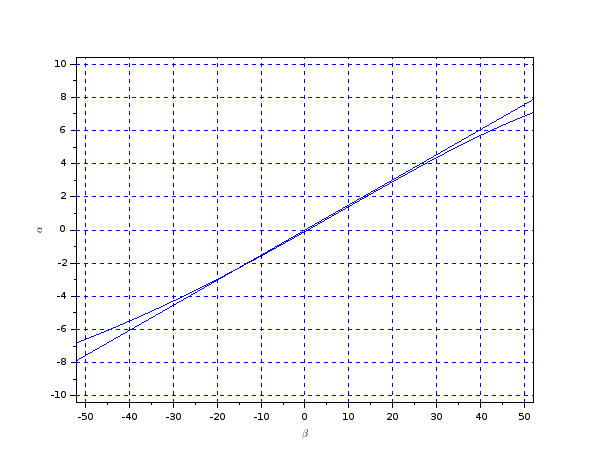
\includegraphics[scale=0.5]{images/plot1.png}

\subsection{2) $\beta = \pm 300$ Grad}
-periodisch